\documentclass{article}
\usepackage{tikz, comment}
\usepackage{pifont}
\usepackage{fontspec, pgfplots}
\usetikzlibrary{arrows, decorations.markings, decorations.pathreplacing}
\begin{comment}
:Title: Not defined yet
:Tags: absolute value rules;properties of equality, equation rules;adjugate, classical adjoint;set;equivalence properties of equality
:Prob: 0.6286;0.5531;0.528;0.4908;0.4871
:Author: Prof.Hu Ji-shan, HKUST
:Slug: No name yet

Description Here.........
\end{comment}
\begin{document}\centering 

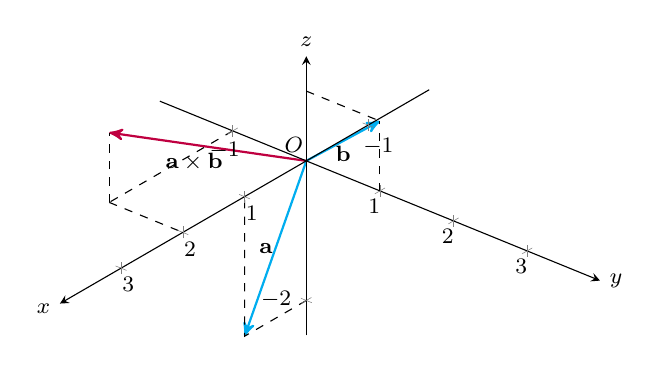
\begin{tikzpicture}[font=\footnotesize]
\pgfplotsset{compat=1.8}
\begin{axis}
[axis lines = center, view={130}{45}, scale=1.5, %ticks=none, 
axis on top, xlabel = {$x$}, ylabel ={$y$}, zlabel ={$z$}, domain =0:1, y domain =0:1,
xmin =-1.99,
xmax =3.99,
ymin =-1.99,
ymax =3.99,
zmin =-2.5, 
zmax =1.5,
samples =10, samples y =40, z buffer =sort,
every axis x label/.style={
    at={(ticklabel* cs:1)},
    anchor= east, yshift =-2
},
every axis y label/.style={
    at={(ticklabel* cs:1)},
    anchor= west,
},
every axis z label/.style={
    at={(ticklabel* cs:1)},
    anchor= south
}]

\node[xshift=3, yshift=-4, label={100:{$O$}}] at (axis cs:0,0,0) {};

\addplot3[cyan, thick, <-, >=stealth'] coordinates
        {(0,0,0) (1,0,-2)};
\node[xshift=6, label={180:{${\bf a}$}}] at (axis cs:0.5,0,-1) {};
\addplot3[dashed] coordinates
        {(0,0,-2) (1,0,-2) (1,0,0)};

\addplot3[cyan, thick, data cs=cart, ->, >=stealth'] coordinates
        {(0,0,0) (0,1,1)};
\node[xshift=0, label={-90:{${\bf b}$}}] at (axis cs:0,0.5,0.7) {};
\addplot3[dashed] coordinates
        {(0,1,0) (0,1,1)};
\addplot3[dashed] coordinates
        {(0,1,1) (0,0,1)};

\addplot3[purple, thick, ->, >=stealth'] coordinates
        {(0,0,0) (2,-1,1)};
\node[xshift=0, yshift=0, label={-45:{${\bf a\times b}$}}] at (axis cs:2,-0.5,1.2) {};

\addplot3[dashed] coordinates%xy-plane
        {(2,-1,1) (2,-1,0) };
\addplot3[dashed] coordinates%y-axis
        {(2,-1,0) (0,-1,0)};
\addplot3[dashed] coordinates%x-axis
        {(2,-1,0) (2,0,0)};
        
\end{axis}

\end{tikzpicture}
\end{document}